% F-16 GNC two-loop architecture overview
% NASA TM-2015-218675  F16_control.dml
\documentclass[tikz, border=4pt]{standalone}
\usepackage{tikz}
\usetikzlibrary{arrows.meta, positioning, shapes.geometric, calc, fit, backgrounds}
\usepackage{amsmath}

\begin{document}
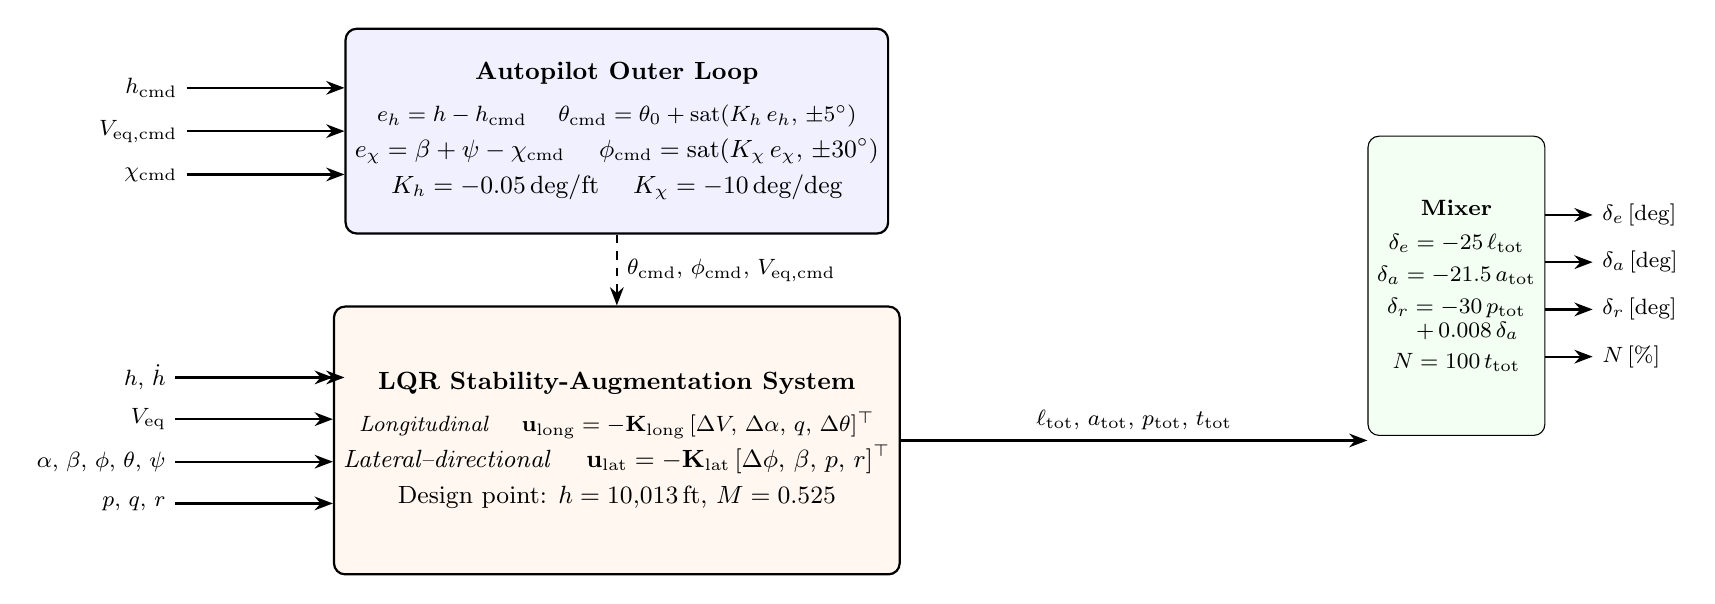
\begin{tikzpicture}[
  >=Stealth,
  every node/.style = {font=\small},
  %-- block styles -------------------------------------------------------
  outerbox/.style = {draw, thick, rounded corners=4pt,
                     minimum width=6.2cm, minimum height=2.6cm,
                     align=center, fill=blue!6},
  innerbox/.style = {draw, thick, rounded corners=4pt,
                     minimum width=6.2cm, minimum height=3.4cm,
                     align=center, fill=orange!6},
  gainblock/.style = {draw, rectangle, rounded corners=2pt,
                      minimum width=1.5cm, minimum height=0.55cm,
                      align=center, fill=white, font=\footnotesize},
  sumnode/.style  = {draw, circle, inner sep=0pt, minimum size=0.55cm,
                     fill=white},
  iolab/.style    = {font=\footnotesize},
  arrow/.style    = {->, thick},
  dasharrow/.style= {->, thick, dashed},
]

% ── Autopilot outer loop box ──────────────────────────────────────────────────
\node[outerbox] (AP) at (0,3.6) {%
  \textbf{Autopilot Outer Loop}\\[4pt]
  \footnotesize
  $e_h = h - h_{\mathrm{cmd}}$ \quad
  $\theta_{\mathrm{cmd}} = \theta_0 + \mathrm{sat}(K_h\, e_h,\,\pm5^\circ)$\\[2pt]
  $e_\chi = \beta+\psi - \chi_{\mathrm{cmd}}$ \quad
  $\phi_{\mathrm{cmd}} = \mathrm{sat}(K_\chi\, e_\chi,\,\pm30^\circ)$\\[2pt]
  $K_h = -0.05\,\text{deg/ft}$ \quad
  $K_\chi = -10\,\text{deg/deg}$
};

% ── LQR SAS inner loop box ────────────────────────────────────────────────────
\node[innerbox, below=0.9cm of AP] (LQR) {%
  \textbf{LQR Stability-Augmentation System}\\[4pt]
  \footnotesize
  \textit{Longitudinal} \quad
  $\mathbf{u}_{\mathrm{long}} = -\mathbf{K}_{\mathrm{long}}\,
    [\Delta V,\,\Delta\alpha,\,q,\,\Delta\theta]^\top$\\[2pt]
  \textit{Lateral–directional} \quad
  $\mathbf{u}_{\mathrm{lat}} = -\mathbf{K}_{\mathrm{lat}}\,
    [\Delta\phi,\,\beta,\,p,\,r]^\top$\\[2pt]
  Design point: $h=10{,}013\,\text{ft}$, $M=0.525$
};

% ── Surface mixer / output ────────────────────────────────────────────────────
\node[gainblock, right=2.8cm of AP, minimum width=2.1cm, minimum height=3.8cm,
      fill=green!5, rounded corners=4pt] (mixer) at
      ($(AP.east)!0.5!(LQR.east)+(3.2,0)$) {%
  \textbf{Mixer}\\[3pt]
  \footnotesize
  $\delta_e = -25\,\ell_{\mathrm{tot}}$\\[2pt]
  $\delta_a = -21.5\,a_{\mathrm{tot}}$\\[2pt]
  $\delta_r = -30\,p_{\mathrm{tot}}$\\[-1pt]
  $\phantom{\delta_r} {+}\,0.008\,\delta_a$\\[2pt]
  $N = 100\,t_{\mathrm{tot}}$
};

% ── Input labels — AP commands ────────────────────────────────────────────────
\node[iolab, left=2.0cm of AP.west, yshift= 0.55cm] (altcmd) {$h_{\mathrm{cmd}}$};
\node[iolab, left=2.0cm of AP.west, yshift= 0.00cm] (veqcmd) {$V_{\mathrm{eq,cmd}}$};
\node[iolab, left=2.0cm of AP.west, yshift=-0.55cm] (chicmd) {$\chi_{\mathrm{cmd}}$};

\draw[arrow] (altcmd.east) -- ++(0.3,0) |- (AP.west|-altcmd);
\draw[arrow] (veqcmd.east) -- (AP.west|-veqcmd);
\draw[arrow] (chicmd.east) -- ++(0.3,0) |- (AP.west|-chicmd);

% ── Input labels — sensor feedbacks ──────────────────────────────────────────
\node[iolab, left=2.0cm of LQR.west, yshift= 0.80cm] (hfb)     {$h,\,\dot{h}$};
\node[iolab, left=2.0cm of LQR.west, yshift= 0.27cm] (vfb)     {$V_{\mathrm{eq}}$};
\node[iolab, left=2.0cm of LQR.west, yshift=-0.27cm] (attfb)   {$\alpha,\,\beta,\,\phi,\,\theta,\,\psi$};
\node[iolab, left=2.0cm of LQR.west, yshift=-0.80cm] (ratefb)  {$p,\,q,\,r$};

\draw[arrow] (hfb.east)    -- ++(0.3,0) |- (LQR.west|-hfb);
\draw[arrow] (vfb.east)    -- (LQR.west|-vfb);
\draw[arrow] (attfb.east)  -- (LQR.west|-attfb);
\draw[arrow] (ratefb.east) -- ++(0.3,0) |- (LQR.west|-ratefb);

% ── AP → LQR (reference states) ──────────────────────────────────────────────
\draw[dasharrow] (AP.south) -- node[right, font=\footnotesize]
                                {$\theta_{\mathrm{cmd}},\,\phi_{\mathrm{cmd}},\,V_{\mathrm{eq,cmd}}$}
                             (LQR.north);

% ── Sensor feedbacks also feed AP (altitude, airspeed) ───────────────────────
\coordinate (mid) at ($(hfb.east)+(0.2,0)$);
\draw[arrow] (mid) |- (AP.west|-altcmd|-mid);

% ── LQR → mixer ──────────────────────────────────────────────────────────────
\draw[arrow] (LQR.east) -- (LQR.east-|mixer.west)
             node[above, font=\footnotesize, pos=0.5]
             {$\ell_{\mathrm{tot}},\,a_{\mathrm{tot}},\,p_{\mathrm{tot}},\,t_{\mathrm{tot}}$};

% ── Mixer outputs ─────────────────────────────────────────────────────────────
\node[iolab, right=0.6cm of mixer.east, yshift= 0.90cm] (el)  {$\delta_e$\,[deg]};
\node[iolab, right=0.6cm of mixer.east, yshift= 0.30cm] (ail) {$\delta_a$\,[deg]};
\node[iolab, right=0.6cm of mixer.east, yshift=-0.30cm] (rdr) {$\delta_r$\,[deg]};
\node[iolab, right=0.6cm of mixer.east, yshift=-0.90cm] (pwr) {$N$\,[\%]};

\draw[arrow] (mixer.east|-el)  -- (el.west);
\draw[arrow] (mixer.east|-ail) -- (ail.west);
\draw[arrow] (mixer.east|-rdr) -- (rdr.west);
\draw[arrow] (mixer.east|-pwr) -- (pwr.west);

\end{tikzpicture}
\end{document}
